\documentclass{beamer}
\usepackage[utf8]{inputenc}

\usetheme{Madrid}
\usecolortheme{default}
\usepackage{amsmath,amssymb,amsfonts,amsthm}
\usepackage{txfonts}
\usepackage{multicol}
\usepackage{tkz-euclide}
\usepackage{listings}
\usepackage{adjustbox}
\usepackage{array}
\usepackage{tabularx}
\usepackage{gvv}
\usepackage{lmodern}
\usepackage{circuitikz}
\usepackage{tikz}
\usepackage{graphicx}
\usepackage{hyperref}
\usepackage{siunitx}

\setbeamertemplate{page number in head/foot}[totalframenumber]

\usepackage{tcolorbox}
\tcbuselibrary{minted,breakable,xparse,skins}



\definecolor{bg}{gray}{0.95}
\DeclareTCBListing{mintedbox}{O{}m!O{}}{%
  breakable=true,
  listing engine=minted,
  listing only,
  minted language=#2,
  minted style=default,
  minted options={%
    linenos,
    gobble=0,
    breaklines=true,
    breakafter=,,
    fontsize=\small,
    numbersep=8pt,
    #1},
  boxsep=0pt,
  left skip=0pt,
  right skip=0pt,
  left=25pt,
  right=0pt,
  top=3pt,
  bottom=3pt,
  arc=5pt,
  leftrule=0pt,
  rightrule=0pt,
  bottomrule=2pt,
  toprule=2pt,
  colback=bg,
  colframe=orange!70,
  enhanced,
  overlay={%
    \begin{tcbclipinterior}
    \fill[orange!20!white] (frame.south west) rectangle ([xshift=20pt]frame.north west);
    \end{tcbclipinterior}},
  #3,
}
\lstset{
    language=C,
    basicstyle=\ttfamily\small,
    keywordstyle=\color{blue},
    stringstyle=\color{orange},
    commentstyle=\color{green!60!black},
    numbers=left,
    numberstyle=\tiny\color{gray},
    breaklines=true,
    showstringspaces=false,
}
%------------------------------------------------------------
%This block of code defines the information to appear in the
%Title page
\title %optional
{12.330}
\date{October 12,2025}
%\subtitle{A short story}

\author % (optional)
{Aditya Appana - EE25BTECH11004}

\begin{document}


\frame{\titlepage}
\begin{frame}{Question}
If a weight of $\vec{P}= 100N$ is supported by two massless strings connected to the walls
as shown in the figure, the value of $T_1$ is \rule{1.5cm}{0.15mm} N. 
\begin{figure}[H]
    \centering
    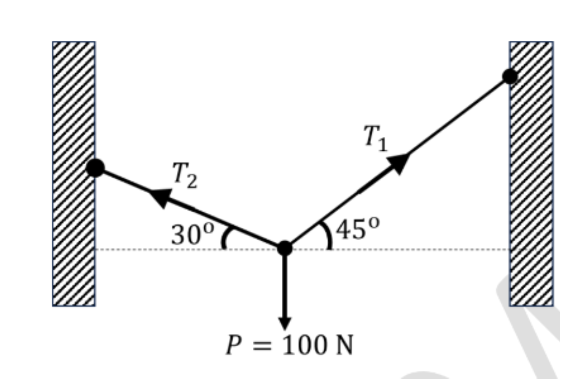
\includegraphics[width=0.4\columnwidth]{Figs/123301.png}
    \caption{Figure}
    \label{fig:placeholder}
\end{figure}
\end{frame}



\begin{frame}[fragile]
    \frametitle{Solution}
\begin{align}
\vec{T_1} + \vec{T_2} = -\vec{P}\\
\vec{T_1} = \norm{T_1}\myvec{\cos 45 \degree \\ \sin 45 \degree}\\
\vec{T_2} = \norm{T_2}\myvec{\cos 180-30 \degree \\ \sin 180-30 \degree} =\norm{T_2}\myvec{\cos 150 \degree \\ \sin 150 \degree} \\
\vec{P} = -\norm{P}\myvec{\cos -90 \degree \\ \sin -90 \degree} = -100\myvec{\cos (-90 \degree) \\ \sin (-90 \degree)}
\end{align}
\end{frame}
\begin{frame}[fragile]
Therefore:
\begin{align}
    \norm{T_1}\myvec{\frac{1}{\sqrt{2}}\\ \frac{1}{\sqrt{2}}} + \norm{T_2}\myvec{-\frac{\sqrt{3}}{2} \\ \frac{1}{2}} = 100\myvec{0\\1} \\
    \myvec{\frac{1}{\sqrt{2}} & -\frac{\sqrt{3}}{2}\\  \frac{1}{\sqrt{2}} & \frac{1}{2}}\myvec{\norm{T_1} \\ \norm{T_2}} = \myvec{0 \\ 100}
\end{align}\\
Organising the data into an augmented matrix and obtaining RREF:
\begin{align}
\myaugvec{2}{ \frac{1}{\sqrt{2}} & -\frac{\sqrt{3}}{2} & 0\\  \frac{1}{\sqrt{2}} & \frac{1}{2} & 100}\xrightarrow{\text{$R_2$ \rightarrow $R_2- R_1$}}
\myaugvec{2}{ \frac{1}{\sqrt{2}} & -\frac{\sqrt{3}}{2} & 0\\ 0 & \frac{1}{2} +\frac{\sqrt{3}}{2} & 100}
\end{align}
\end{frame}


\begin{frame}[fragile]
    \frametitle{Solution}
\begin{align}
    \norm{T_2} = \frac{200}{1+\sqrt{3}} = 73.205N\\
    \norm{T_1} = \frac{\sqrt{3}}{\sqrt{2}}\norm{T_1} = 89.658N
\end{align}
\end{frame}

\begin{frame}[fragile]
    \frametitle{Code}
\begin{lstlisting}
import numpy as np
import numpy.linalg
import matplotlib.pyplot as plt
import math

matrix = np.array([[math.cos(math.pi/4), math.cos(5*math.pi/6)],
                   [math.sin(math.pi/4), math.sin(5*math.pi/6)]])

vec = np.array([0,100])

norms = np.linalg.solve(matrix,vec)

print(norms)

fig = plt.figure(figsize = (10,10))
ax = fig.add_subplot(111)
\end{lstlisting}
\end{frame}
\begin{frame}[fragile]
    \frametitle{Code}
\begin{lstlisting}

ax.axhline(y=0, color='k')
ax.axvline(x=0, color='k')

ax.quiver(0,0,0,-100, color = 'Blue', label = 'P = 100N',  angles='xy', scale_units='xy', scale=1)
ax.quiver(0,0, norms[0]*matrix[0,0], norms[0]*matrix[1,0], color = 'green', label = f"$T_1 = ${round(norms[0],2)}N",  angles='xy', scale_units='xy', scale=1)
ax.quiver(0,0, norms[1]*matrix[0,1], norms[0]*matrix[1,1], color = 'orange', label = f"$T_2 = ${round(norms[1],2)}N",  angles='xy', scale_units='xy', scale=1)


ax.set_xlim(-100, 100)
ax.set_ylim(-100, 100)
ax.legend()
ax.grid(True)
plt.show()
\end{lstlisting}
\end{frame}

\begin{frame}[fragile]
    \frametitle{Figure}
\begin{figure}[H]
    \centering
    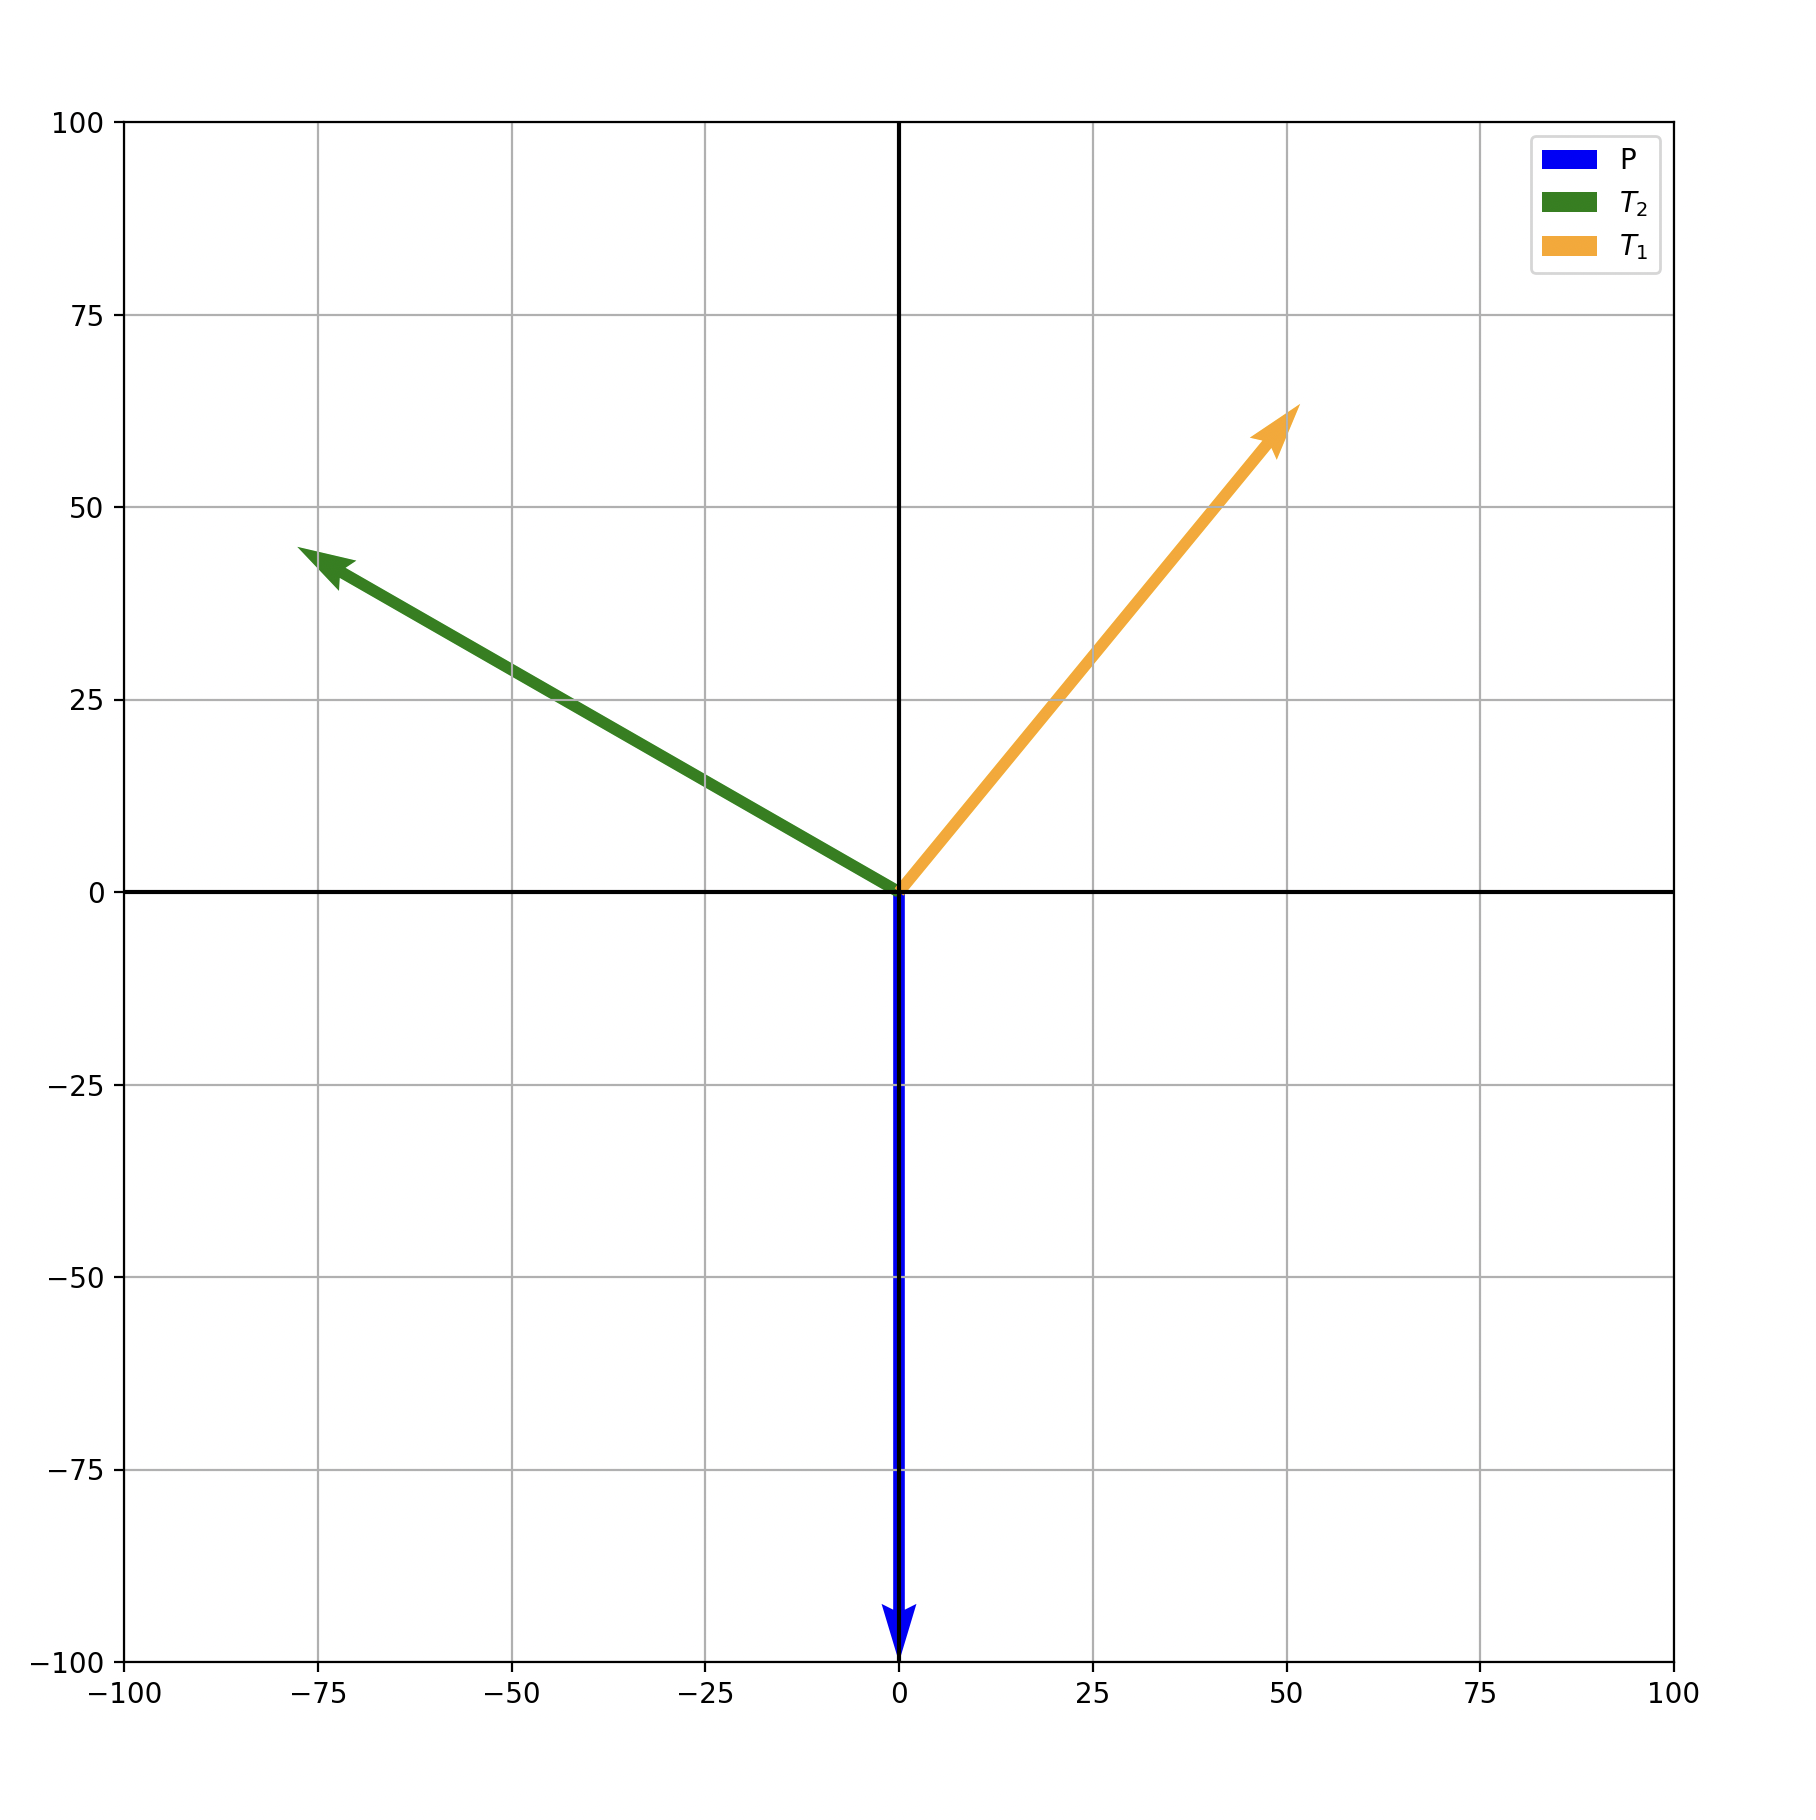
\includegraphics[width=0.6\columnwidth]{Figs/123302.png}
    \caption{Plot}
    \label{fig:placeholder}
\end{figure}
\end{frame}

\end{document}